\chapter{调研工作与源码解析}

对于 Android 应用中图形的绘制体系的优化,需要深度对底层源码进行调研,然后才能上手进行优化。因此开展了流畅性优化调研工作,阅读 Android Framework 以及 Android SDK 的源码,总结出整体的应用绘制体系。在有了这些前置知识的情况下,进行针对 RecyclerView 的优化工作,并搭建合理的流畅性指标来量化优化结果。具体来说,需要对 Android 的绘制体系 —— View 有一定的了解;同时对于 Android 应用对触摸消息的处理以及 Android 消息机制也要有所了解。这些都是 Android 应用程序运行的根本。

\section{Android 绘制体系}

\subsection{View 的测量、布局和绘制}

在 Android 应用程序中,展示 UI 界面以及和用户进行交互的最主要的组件就是 View。View 本身是一个非常复杂的绘制框架,封装了一系列与屏幕刷新相关的操作。开发开发者可以使用 Android SDK 中提供的 View,或者针对具体的业务自定义一些 View 来进行界面的展示,业务逻辑交互的处理操作。对于一个 View 来说,最重要的生命周期有测量(measure)、布局(layout)和绘制(draw)\cite{rountev2014static}。

在测量的过程中,需要确定每一个 View 所占据的矩形区域的大小。其中最典型也是最耗时的就是文本类型的 View 的测量。这些文本因为语言、字符宽度、文字方向等不同的因素,需要进行非常复杂的测量流程,最终才能确定文本的长和宽。因此,View 的测量流程通常也是 View 进行绘制的时候最耗时的一个过程。

在布局过程中,需要根据每一个 ViewGroup 规定的布局方式对其中的子 View 进行布局,也就是确定其在 Window 上显示的位置。常见的 ViewGroup 有线性布局 LinearLayout,帧布局 FrameLayout和相对布局 RelativeLayout 等。这些不同的布局对于其中的子 View 有不同的布局要求,并在真正布局的时候按照这个要求确定子 View 应该摆放的位置。

最后一步就是绘制了,也就是真正将图形绘制到屏幕上的操作。这部分工作大部分是通过 Android 的上层渲染组件 Canvas 来完成的。 Canvas 会将各种类型的图形在 CPU 上进行计算,之后会将这些计算好的结果发送给 GPU 进行渲染。这也是大部分 Android 动画实现的原理。

\begin{figure}
    \centering
    \begin{adjustbox}{max width=\textwidth}
        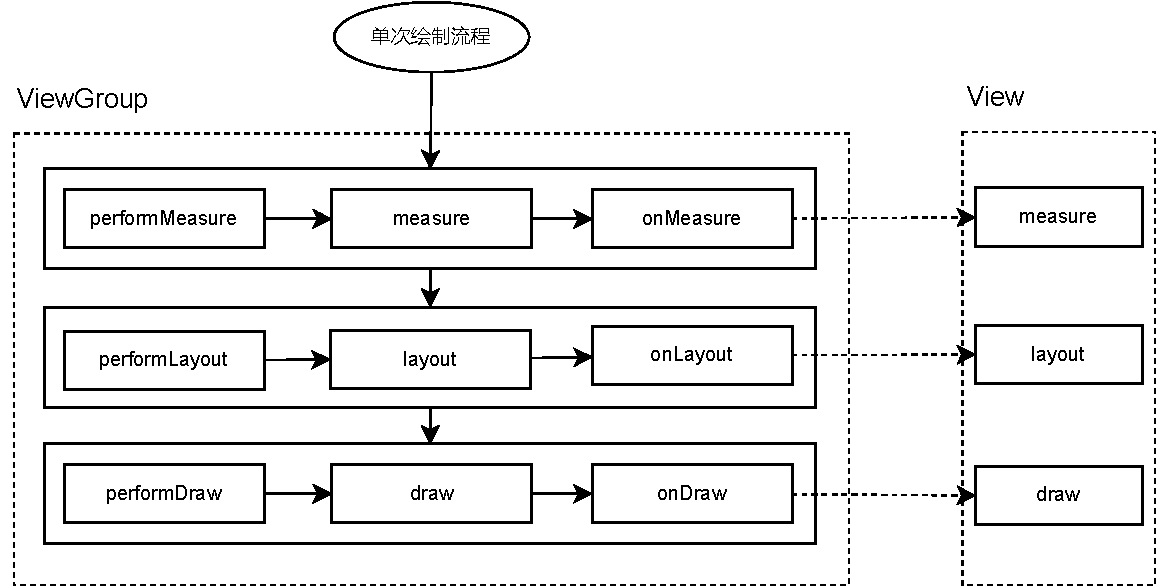
\includegraphics{assets/view-measure-layout-draw.pdf}
    \end{adjustbox}
    \caption{View 的绘制流程}
\end{figure}

对于 ViewGroup 来说,测量的流程需要特别强调。因为 ViewGroup 本身没有内容,它的作用是承载子 View。所以,ViewGroup 的主要测量过程就是去测量自己的子 View,并最终得到所有子 View 的综合属性。大致的 ViewGroup 与 View 配合进行绘制的流程见图 2.1。

然而,View 体系并没有限制 ViewGroup 应该在测量的时机一定得到子 View 的准确测量结果。这就意味着我们可以在测量的时候返回一个假值,并在后面的时机得到真正的值。RecyclerView 就是这样做的。因为它通常需要承载大量的子 View,因此它对于性能的要求非常高。所以它的测量流程作为非常耗时的一个流程,需要尽可能地减少测量的总次数以及避免重复测量。RecyclerView 真正测量子 View 是在布局流程中,在测量完子 View 之后会立刻对子 View 进行布局。这种方式能够避免子 View 在不适宜的时机请求父 View 测量而导致性能下降的问题。当 RecyclerView 在进行布局时,它会禁止子 View 进行布局请求,从而拦截子 View 的测量请求,从而减少不必要的测量次数。

% 这部分之后会在 4.2 详细说明。

\subsection{用户输入事件的处理}

当用户用手触摸屏幕时,触摸行为会定位到特定的 View 上。但是,这个触摸行为只会在下一帧到来时进行响应。因为受限于屏幕的刷新率,只有在下一帧屏幕才能给出新的图像。触摸事件主要有以下几种:

% 所以等到 Choreographer 接收到下一个 VSync 信号时,新的绘制流程启动,这些积累的触摸事件就会在这个时候被消费。

\begin{itemize}
    \item ACTION\_DOWN:用户手指按在屏幕上的事件;
    \item ACTION\_MOVE:用户手指在屏幕上滑动的事件;
    \item ACTION\_UP:用户手指从屏幕上抬起的事件;
    \item ACTION\_CANCEL:当事件被上层 ViewGroup 拦截之后,下层 View 接收到的事件。
\end{itemize}

\begin{figure}[htbp]
    \centering
    \begin{adjustbox}{max width=\textwidth}
        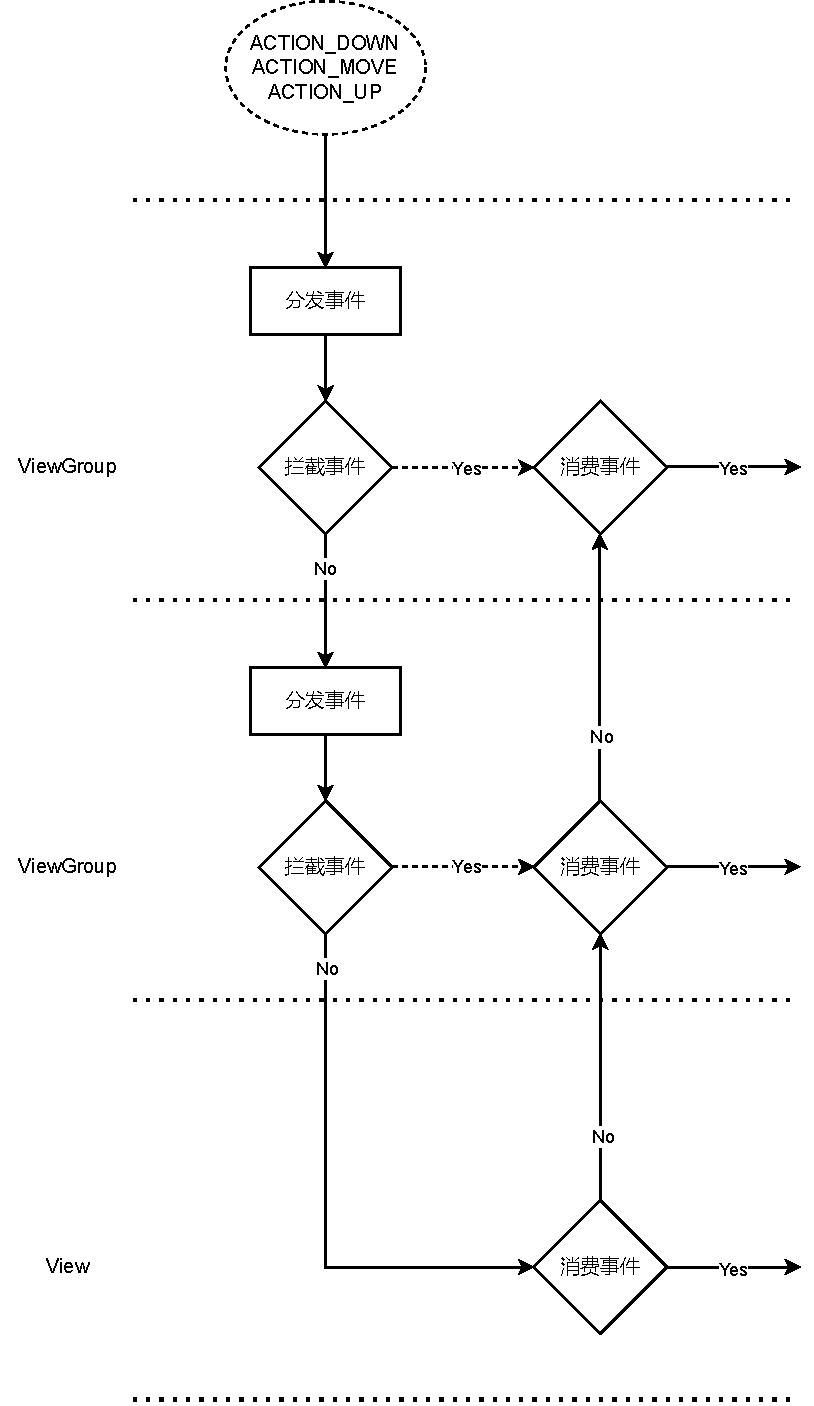
\includegraphics[scale=0.7]{assets/view-touch-event.pdf}
    \end{adjustbox}
    \caption{View 的触摸事件传递流程}
\end{figure}

触摸事件会从 View 树的根节点开始向下传递。事件在链路中流动的路线总体上呈现出“U 型”,如图 2.2。在从顶层的 View 开始向下进行事件的分发(Dispatch)。在这个过程中,路径上的每一个 ViewGroup 都可能拦截(Intercept)这个事件\cite{wu2017appcheck}。如果事件已经传递到了最底层的 View,又或者被其中的某一个 ViewGroup 成功拦截,那么将会由相应的 View 或者 ViewGroup 去逐一消费这个事件。如果事件被当前 View 或 ViewGroup 消费,那么事件的传递将在此终止;如果没有被消费,那么事件会向上传递,直到再次传递到根 View 为止。

对于 RecyclerView 来讲,因为其需要处理大量的滚动操作,所以触摸事件的处理尤为重要。当触摸事件被 RecyclerView 拦截时,它会通过当前是否是滚动状态而选择是否拦截该事件。如果是 ACTION\_MOVE 事件,RecyclerView 通过解析事件的详细信息,发现此时用户触发了滚动操作,那么就会将自己标记为滚动状态,并最终拦截这个 ACTION\_MOVE 事件。因此,之后的事件消费也是由 RecyclerView 自身来进行(嵌套滚动不适用于这段说明,但其不在本文的讨论范围内);如果是 ACTION\_DOWN 事件,那么 RecyclerView 不会拦截这个事件,让其成功到达子 View,由子 View 来决定是否消费该事件。这个过程中,子 View 是否消费 ACTION\_DOWN 事件对后续的事件传递影响尤为重要。如果处理不当,可能会产生一些影响很重大的缺陷。

% 这部分会在 5.4.1 详细说明。

\subsection{Android 消息机制}

Android 应用程序运行的基本框架就是基于消息机制,同时绘制行为和消息机制的配合也非常紧密。Android 系统应用内部的消息机制主要和这几个类相关:Looper、Handler 和 MessageQueue。

Android 系统的主线程对应的类是 ActivityThread。该类内部维护着主线程启动,并处理各个线程发送消息的流程,同时也负责 UI 的绘制消息的处理。当该线程启动时,同时会准备自己的 Looper 来负责消息队列的管理和任务的委派。ActivityThread 中的 Looper 成为 Main Looper。由于只能由主线程来处理 UI 类型任务的分发,所以 Main Looper 也只允许主线程持有。如果应用内部的线程也想利用这套消息机制来进行任务处理(比如埋点上报的线程),也可以准备自己的 Looper 来接收任何线程发送给当前线程的任务并添加到消息队列中,在某一个时刻被取出并执行。

Looper 内部管理的消息队列的实现类就是 MessageQueue。其内部管理了任务队列的管理操作,包括入队、出队,以及空闲时的敏捷任务处理操作等。大部分是通过调用 Android Native 的 C++ 代码来实现,并通过 JNI 包装成面向 Android Framework 以及 Android 应用程序的接口。

Android 程序中,消息不能直接通过访问 Looper 或者 MessageQueue 的方式进行提交,只能通过封装好的方式 —— Handler 进行提交。这种方式更加安全和方便,也能给应用的架构设计提供更好的开发范式。在任何线程中都可以创建 Handler,但是 Handler 在构造的时候必须指定 Looper,也就是明确提交的任务需要由哪一个线程的 Looper 来管理\cite{fan2018efficiently}。同时,Handler 也提供了多种任务执行的方式、多种提交任务的方式以及延时和取消等功能。例如,我们可以在发送一个任务之前,取消之前已经提交但未执行的特定类型的任务来满足特定的业务需求。在对 RecyclerView 的布局流程进行改造时,我们也会利用到这一特性。

\section{Feed 流概念及现状}

目前,越来越多的互联网产品在移动端上增加“短视频”功能,如快手、抖音、美团、西瓜视频、小红书等等,并且短视频板块在这些应用中通常都处于启动的默认引导场景,即 Feed 流,是整个应用平均消费时间最长的板块。因此,这部分的流畅性体验对于用户的留存,消费时长等指标至关重要。能够优化视频起播的速度、滑动的流畅度、网络请求速度等任何一个场景,都能带来非常大的业务收益。本节主要针对基于 RecyclerView 搭建的短视频场景的 Feed 流进行流畅性的优化。因此,首先需要对 RecyclerView 的具体情况进行调研,才能从中找出可以优化的点。

\subsection{RecyclerView 介绍}

RecyclerView 最早在 Google I/O 2016 被提出,用来解决传统应用程序中使用 ListView 处理复杂的列表时带来的性能问题。RecyclerView 本身也是一个 ViewGroup,与其它常用的 ViewGroup,如 ScrollView、ViewPager、ListView 等在绘制流程中的行为是几乎一致的\cite{mawlood2022listview}。只不过,RecyclerView 更加专注于在流式布局的场景下,对于多种复杂的子项进行合理的回收和复用,从而在不断滑动的过程中,增加已有组件的利用率,提高滑动时的性能和流畅度。

RecyclerView 不是单独的一个组件。由于处理各种子 View 的回收和复用,以及处理动画、数据绑定等操作的逻辑都非常复杂,因此将这些逻辑都分成独立的部分。整个 RecyclerView 家族主要由以下几个组件组成:

\begin{itemize}
    \item RecyclerView:父 View 本身,负责响应原有的 View 绘制流程,作为其它组件行为的发起者;
    \item LayoutManager:负责 RecyclerView 的测量和布局流程,安排子 View 的位置。有不同的实现方式,比如线性布局,网格布局等等。本文中主要考虑在 Feed 流场景下常见的线性布局 LinearLayoutManger;
    \item ItemAnimator:负责子 View 的显示,隐藏等动画。因为不涉及到核心的布局流程,所以本文不涉及到这方面的优化;
    \item Adapter:RecyclerView 最核心的数据管理类。所有的子 View 中的数据由 Adapter 来管理,并在合适的时机进行绑定,从而能够显示在屏幕上。Adapter 作为数据的存储器,能够通知 RecyclerView 数据发生了何种变化,从而通知 RecyclerView 进行适当的刷新操作。
\end{itemize}

接下来将通过对 RecyclerView 本身的测量、布局、滑动、数据处理流程来认识这些组件,并引出相应的优化点。

\subsection{RecyclerView 的测量}

对于一个 ViewGroup 来说,它的测量过程就是要知道自己所有的子 View 的综合属性。然而,如果 RecyclerView 本身无法知晓子 View 都有谁,那自然无法进行测量。和其它的布局(如 LinearLayout,FrameLayout 等)不同,其它的布局在创建的时候,无论是通过 XML 还是手动在代码中调用 addView() 来创建,都是已经知道子 View 的完整状态;而 RecyclerView 获取子 View 参数信息的手段是通过 Adapter。而 Adapter 最重要的数据准备过程是交给开发者来决定的。因此,在初次测量时,RecyclerView 拿不到任何子 View 的信息。这个时候,如果RecyclerView 在布局方向(垂直或水平)上的属性是固定的值,那么测量就会很简单,直接返回对应的值即可;如果是一个不确定的值(比如 WRAP\_CONTENT),那么会先尝试进行一次布局流程,然后再进行测量。通常情况下, RecyclerView 在布局方向上的长度都是一个固定的值,因为这样能够很大程度上减少重复测量的次数,从而提高滑动的性能。

\subsection{RecyclerView 的布局}

布局是 RecyclerView 最关键的流程。这里涉及的就是对Adapter的消费,布局其中的子 View,以及回收和复用发生的地方。布局操作的整个流程在方法 dispatchLayout() 中,里面的流程分为三步。这三步所做的事情如下:

\begin{itemize}
    \item 第一步:处理 Adapter 中提交的更新,同时保存当前子 View 的参数信息;
    \item 第二步:对于每一个子 View,执行最终的测量和布局流程,确定它们安放的位置。这个过程也是 RecyclerView 和 Adapter 交互最主要的过程 —— 进行数据绑定;
    \item 第三步:主要处理动画的流程。因为不涉及到布局上的性能优化,本文不进行讨论。
\end{itemize}

接下来,我们将对 RecyclerView 最主要的布局流程进行分析。首先,RecyclerView 会拦截子 View 对布局的请求。在 RecyclerView 布局的过程中,子 View 本身就已经将要被布局,因此 RecyclerView 认为在这个时刻任何子 View 的布局请求都是多余的。RecyclerView 并不会允许子 View 在这个时候请求布局。等到第三步结束之后,才再次允许子 View 进行布局请求。实际上,在真实开发过程中,也非常不建议在 RecyclerView 的子 View 中手动进行布局请求,而是使用 Adapter 去通知的方式进行增量更新。这样会有更高的效率和更安全的执行流程。

核心布局流程可以简单概括为:计算出起始锚点(通常是延布局方向的起始位置),并沿着布局方向决定每个 View 的行为。有可能是创建新的 View,也有可能是复用之前回收的 View;并给这些确定会显示在屏幕上的 View 进行数据绑定。这个过程中,创建和绑定的操作是交给 Adapter 来完成的。也就是说,开发者需要在自己的 Adapter 中完成创建和绑定的流程。因此,这个过程中我们能够进行一些特殊的操作。比如提前拿到 View 进行绑定,甚至利用空闲时间异步创建出 View 来避免真正用到 View 时才去创建而导致耗时增加;另外要强调的一点是,由于 View 本身不能具有 RecyclerView 需要的准确的参数信息(位置信息,状态变化标记位等),同时也不能被妥善地回收和复用。因此 RecyclerView 框架的做法是在 View 上包装一层 ViewHolder 来持有 View 的引用。对于 LayoutManager 来说,它直接操作的是 ViewHolder 而非 View,这样能够更好地对 View 进行回收和复用,也便于增加一些位置变化等关键信息来让 LayoutManager 更迅速地进行布局操作。

% \subsection{RecyclerView 对于滑动过程的处理}

% 任何 View 处理滑动流程时,都需要处理 ACTION\_DOWN 事件、ACTION\_MOVE 事件和 ACTION\_UP 事件。通常,一个完整的滑动流程是一个 ACTION\_DOWN 加上若干个 ACTION\_MOVE 以及结尾的 ACTION\_UP。因此,对于 RecyclerView 来说,如何处理 ACTION\_DOWN 事件的走向尤为重要,这影响了后续事件的分发,自然也影响了整个的滑动流程。当 ACTION\_DOWN 事件产生时,RecyclerView 并不会拦截该事件,只会将事件传递给子 View。而子 View 可以自主选择是否消费该事件。如果子 View 没有消费 ACTION\_DOWN,那么将会由 RecyclerView 自己来消费。RecyclerView 本身永远会消费任何触摸事件,所以无法再继续向上传递。之后所有的 ACTION\_MOVE 事件以及最后的 ACTION\_UP 事件都会由 RecyclerView 自己来消费。这也是滑动流程中最理想的情况,完全由 RecyclerView 来主动控制。

% 但是,通常 RecyclerView 的子 View 是需要消费 ACTION\_DOWN 事件的。比如一个可以点击的新闻条目、一个视频条目等等。这些响应了点击事件的子 View 自然需要消费 ACTION\_DOWN 事件来处理点击过程。这也就导致了接下来的 ACTION\_MOVE 事件并不会被发送给 RecyclerView 来消费。那么在这种情况下,RecyclerView 应该如何处理滑动流程呢?答案是通过拦截。虽然 RecyclerView 接下来不会收到子 View 传递来的未经过消费的 ACTION\_MOVE 事件,但是在将其传递给子 View 之前,RecyclerView 本身也可以拦截该事件。因此,RecyclerView 在拦截的流程中,只要发现当前事件是 ACTION\_MOVE 事件,就会设置滑动状态的标记位,并拦截该事件。结果就是子 View 会收到 ACTION\_CANCEL 事件从而无法进行滑动处理(不进行嵌套滑动处理的条件下),而 RecyclerView 本身能够通过该方式消费 ACTION\_MOVE 事件以及最后的 ACTION\_UP 事件。虽然这样确实能够保证 RecyclerView 正常处理滑动流程,但是和直接处理不同,如果是通过拦截的方式处理 ACTION\_MOVE 事件,拦截的过程和真正进行滑动的过程会位于两个不同的消息,也就是两个不同的流程中。这样会导致如果中间被其他消息插入,会产生一些副作用。这部分也是我们在优化过程中需要重点克服的困难之一。

% 在真正进行滑动的过程中,会对每一次滑动事件进行解析。解析出的滑动距离、方向等属性会用于接下来的布局过程。RecyclerView 会对因为滑动而改变的子 View 进行重新的测量和布局,并尽可能复用已经被回收的 ViewHolder 来减少重复创建。对于新添加的子 View,也会通过 Adapter 进行数据绑定。

\subsection{RecyclerView 对数据改动的响应}

RecyclerView 最推荐的方式是进行增量更新,而不是全量更新。全量更新会导致 RecyclerView 整体的刷新,同时会将所有已经位于屏幕上绑定数据完成的 View 进行回收和废弃,接下来会重新用新的数据进行绑定。因此,如果真正的修改只有非常小的一部分,建议通过增量更新的方式通知 RecyclerView,之后在 RecyclerView 的布局阶段的第一步中会消费这些更新请求,并在最终布局的流程中只进行修改部分的重新布局。这对于性能的提升很大,同时也为动画的执行留足了 CPU 资源。

数据改动的通知是通过 Adapter。当需要的数据发生变化时,会先修改 Adapter 持有的数据结构,并调用 Adapter 的接口去通知 RecyclerView 发生了什么样的变化。这些改动统一被包装成接口,调用即可提交改动至 RecyclerView。而 RecyclerView 本身通过观察者模式观察 Adapter 中的数据变化。每一次改动行为都会被存放到队列中进入代办(Pending)状态,直到布局流程开始时会被消费。在消费的过程中,也只会通过改动中提交的位置信息对可能受影响的子 View 进行修改。

\subsection{视频类型 Feed 流}

在视频类型 Feed 流的场景下,通常 RecyclerView 的一个子 View 作为一个视频的载体。当用户向下滑动时,下一个视频由于被滑动到屏幕内,会进行布局和数据绑定,从而显示在屏幕上。这里面主要的信息有视频的封面图片、视频标题、作者信息等等。从用户的感官角度看,当该子 View 被滑动到屏幕中央定位完毕时,视频会进行播放,此时用户可以对视频的进度,播放速度等进行控制。同时能够通过点赞、评论、收藏等方式进行交互。

% 对于下一个视频信息的加载过程,通常是需要格外小心的。因为该过程发生在用户滑动屏幕的时候,此时主线程正不断接受用户发送的滑动事件,并根据这些滑动的事件来进行布局、UI 刷新等操作,占据了主线程很大一部分资源。如果这个时候数据绑定的流程过于复杂,会严重增加这段时间的主线程耗时,从而影响整体的流畅性,甚至造成肉眼可见的卡顿。因此,在 Adapter 进行数据绑定的过程中,是强烈不建议在主线程进行任何耗时任务的。这些任务要么通过异步的方式后续补齐,要么针对具体的业务,寻找合适的时机提前进行。

% 然而,经过业务的不断迭代,数据绑定的耗时一定会随着业务方不断添加新的功能而增加。因此,我们希望能够对这个过程进行彻底的优化。也就是能够在一个合适的时机将整个数据绑定操作提前进行,而不是只异步化其中的一小部分。在视频 Feed 流的场景中,合适的时机是比较容易寻找的,因为用户在滑动到一个视频之后通常会停留一段时间进行交互行为。但是这样的行为会让 RecyclerView 的生命周期产生混乱,因此即使能够做到,也需要经过细致的修复来让其能够准确地派发原先的生命周期。

通过对公司内的线上应用,传统的利用 RecyclerView + SnapHelper 来开发视频类型应用的范式,以及网络上开源的视频应用开发手段得出,基于 RecyclerView 所搭建的视频类型 Feed 流,通常需要进行如下定制:

\begin{enumerate}
    \item 将 RecyclerView 的缓存关闭,因为会影响生命周期派发,导致业务埋点上报混乱;
    \item 将 LayoutManager 的预取功能关闭,该功能会影响数据绑定的生命周期派发。
\end{enumerate}

接下来详细说明这两个功能需要关闭的原因。RecyclerView 的缓存机制是一种对离开屏幕的数据的暂时保护。当一个子 View 因为滑动而脱离屏幕可见范围时,理论上应该被回收,并用于接下来新出现的 View 的数据绑定。但是用户也有可能会重新向反方向滑动,让这些 View 重新显示在屏幕上。因此将这些暂时脱离屏幕的 View 放入缓存中,能够让这些数据保存下来避免被回收,这样重新显示时就不需要再次进行绑定,从而提高流畅性;然而,对于视频类型的应用来说,用户向上滑动的操作数量会少很多,反映到数据上就是 RecyclerView 的缓存命中率非常低。同时,由于增加了缓存,在 View 重新显示时不需要进行数据绑定,开发者也没有任何手段通过 SDK 获知 View 从缓存中被取出的时机。因此这些 View 的曝光埋点也就无法进行上报。所以对于视频类型的 Feed 流,缓存通常会被关闭,当 View 重新显示时依然进行绑定操作。业务方会依赖这些绑定事件,在进行数据绑定的同时上报曝光埋点,表示该子 View 已经对用户可见,代表着一次用户的消费行为;LayoutManager 的预取功能需要关闭也是同样的原因。预取会导致接下来即将出现的 View 被提前绑定,从而让曝光埋点错误上报。因为我们没有一个比较好的时机去确定当前 View 是否对用户可见,所以只能选择最接近的绑定时机。

在这样的条件下,只有当卡片因为用户滑动屏幕而出现在屏幕内时,才会进行数据绑定。这虽然能满足企业通过收集埋点来统计用户消费情况的需求,但是也会导致从用户的滑动行为开始到视图真正对用户可见的过程中出现可感知的耗时。这段时间越长,用户就越容易产生卡顿的感觉。